\section{Belief Propagation} \label{BP}

Warning Propagation braucht bisher 2 Seiten, in der fertigen Version also etwa 4-5. Belief Propagation sollte in etwa den selben Umfang haben, etwas weniger Beschreibung nötig weil vieles gleich ist, dafür aber komplizierter.

\begin{itemize}

\item[Algorithmus] In \ref{BPA} Algorithmus beschreiben. Grundsätzliche  Vorgehensweise ist dieselbe wie WP, also "nur" unterschiedliche Arten von Nachrichten und neue Update-Regel beschreiben

\item[Lösungen] Hier zeigen, wie  die Anzahl der erfüllenden Belegungen und die Wahrscheinlichkeit für $x_i = 1$ aus den konvergierten Nachrichten berechnet wird. Wenn noch genug Seiten frei mit ausführlichem Beispiel

\end{itemize}

\subsection{Propagation Algorithm} \label{BPA}

\subsubsection{Messages}
The messages sent in the BP algorithm are conditional probabilities $\mu \in [0, 1]$. The corresponding events are taken from the probability space of all SAT assignments that satisfiy. The probability measure is a uniform distribution so for a SAT formula over $n$ variables each assignment has probability $2^{-n}$.

The messages $\mu_{a \rightarrow i}(x_i)$ sent from a factor $a$ to a variable $i$ is the probability that $a$ is satisfied conditioned on $i$ taking the value $x_i$. 

The message $\mu_{i \rightarrow a}(x_i)$ sent in the opposite direction is the probability that $i$ takes the value $x_i$ in an assignment that satisfies $\tau_{i \rightarrow a}$.

\begin{example}
Let $\mathcal{F} = \underbrace{(x_1 \lor x_2)}_a \land \underbrace{(\overline{x_1} \lor \overline{x_3})}_b \land \underbrace{x_3}_c $.
\end{example}
\begin{figure}[h]
\centering

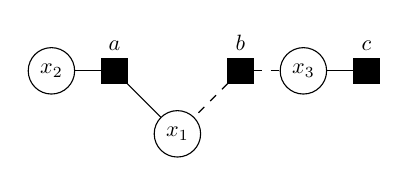
\begin{tikzpicture}[scale=0.8,transform shape]
   	\node[rectangle,draw=black, label = {$a$}, fill] (a) at (0,0) {$a$};
   	\node[rectangle,draw=black, label = {$b$}, fill] (b) at (2,0) {$a$};
   	\node[rectangle,draw=black, label = {$c$}, fill] (c) at (4,0) {$a$};
   
  \node[shape=circle,draw=black] (x1) at (1,-1) {$x_1$};
   
  \node[shape=circle,draw=black] (x2) at (-1,0) {$x_2$};
  \node[shape=circle,draw=black] (x3) at (3,0) {$x_3$};
 


    
	\draw[-] (a) edge [right] node {} (x1);
	\draw[-] (a) edge [right] node {} (x2);
	\draw[-, dashed] (b) edge [right] node {} (x1);
	\draw[-, dashed] (b) edge [right] node {} (x3);
	\draw[-] (c) edge [right] node {} (x3);

\end{tikzpicture}
\end{figure}
In this example, the values of $\mu_{c \rightarrow 3}(1), \mu_{b \rightarrow 3}(1), \text{ and }\mu_{1 \rightarrow a}(1)$ are computed using only their definition: \newline For $c$ to be satisfied, $x_3$ has to take the value $1$, so $\mu_{c \rightarrow 3}(1) = 1$. The value of $\mu_{b \rightarrow 3}(1)$ can be obtained by dividing the number of assignments with $x_3 = 1$ that satisfy $b$ by the number of all assignments with $x_3 = 1$. If $x_3 = 1$, $x_1$ has to set to $0$, so out of all $4$ assignments with $x_3 = 1$ there are $2$ that satisfy b: $\mu_{b \rightarrow 3}(1) = 0.5$.
 
The value of $\mu_{1 \rightarrow a}(1)$ is the fraction of $(1, \star, \star)$-assignments that satisfy $b$ and $c$. The satisfying assignments are $(1,0,1)$ and $(0,0,1)$ so  $\mu_{1 \rightarrow a}(1) = 0.5$.

\subsubsection{Update Rules}

The probability $\mu{i \rightarrow a}$ is the probability that $i$ takes the value $x_i$ if all clauses except $a$ are satisfied. Since it is assumed, that $\mathcal{F}$ is satisfiable 

\begin{figure}[h]
\centering

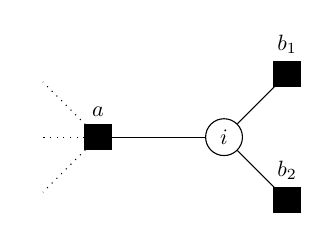
\begin{tikzpicture}[scale=0.8,transform shape]
   	\node[rectangle,draw=black, label = {$a$}, fill] (a) at (0,0) {$a$};
   	
\node[shape=circle,draw=black] (i) at (2,0) {$i$};   	
   	
   	\node[rectangle,draw=black, label = {$b_1$}, fill] (b1) at (3,1) {$a$};
   	\node[rectangle,draw=black, label = {$b_2$}, fill] (b2) at (3,-1) {$a$};

	\node[] (x1) at (-1,0) {};
	\node[] (x2) at (-1,1) {};
	\node[] (x3) at (-1,-1) {};

    \draw[dotted] (a) edge [right] node {} (x1);
    \draw[dotted] (a) edge [right] node {} (x2);
    \draw[dotted] (a) edge [right] node {} (x3);
	\draw[-] (a) edge [right] node {} (i);
	\draw[-] (i) edge [right] node {} (b1);
	\draw[-] (i) edge [right] node {} (b2);

\end{tikzpicture}
\end{figure}
\subsection{Marginal Propabilities}

\subsection{Number of satisfying assignments}